\chapter{Experiments with Deep Domain Adaptation}
\label{exp_chapter}

In previous chapters, we have selected suitable astronomical data
and surveyed and choosen suitable deep domain adaptaion methods.
Now, we carry out experiments with the selected methods
on astronomical spectra from the SDSS and LAMOST spectroscopic sky surveys.

Firstly, we create source and target datasets for experiments.
Then, we reduce the data to two-dimensions
so we are able to visualise the data
and investigate distributions of both the source and target data.
% TODO CNN abbreviation
Thirdly, we introude a CNN baseline model
which serves as benchmark for comparison of deep domain adapation methods.
Finally, we employ four deep domain adaptation methods
(DDC, Deep CORAL, DANN and DRCN)
and evaluate the adapted results to see 
if astronomical spectroscopy can benefit from deep domain adaptation.

\section{Data Preparation}

% TODO introduction to section

Our data of source domain consists of 4\,851\,200 optical spectra from the SDSS DR14 catalog
and the corresponding SDSS DR14Q catalog of 649\,791 spectra of 526\,356 QSO objects
(we have to distinguish an object and a spectrum
because each astronomical object could be observed multiple times
having more spectra).
Both catalogs are introduced in~Subsection~\ref{sdss}.
However, 20\,279 spectra of QSOs cannot be idenfified
% TODO describe the bug in SDSS DR14Q catalog
because there is a bug in the SDSS DR14Q catalog.
Therefore, we are able to identify only 629\,512 spectra of all QSOs.
% TODO describe that spectra are stored in individual FITS
% TODO spectra are downloaded according to SDSS DR14 catalog
% TODO lite versions extracted COADD
Next, we need to cross-match the SDSS DR14 and DR14Q catalogs
to merge the data stored in individual FITS files with QSO labels.
The cross-matching is based on triplet of
\textit{plate number}, \textit{Modified Julian Date of obesrvation} and \textit{fiber number} that is unique to each spectrum.
Additionally to the 20\,279 spectra of QSOs lost due to the bug in the DR14Q catalog,
we were unable to cross-match 55 QSOs with the SDSS DR14 catalog.
Therefore, totally we have 629\,457 spectra of QSOs
for which we have actual data in FITS files and not only metadata in catalogs.

Complement to the source domain in domain adapation is the target domain.
We selected data from LAMOST DR5 to be target domain data
for reasons described in Subsection~\ref{lamost}.
The LAMOST DR5 general catalog contains 9\,026\,365 spectra
and the most complete catalog of QSOs has 42\,552 spectra.
Again, we cross-matched the LAMOST DR5 catalog and the catalog of QSOs
according to quartet of \textit{plan identifier}, \textit{local Modified Julian Date} (one less the Modified Julian Date), \textit{spectrograph identifier} and \textit{identifier of fiber}.
We were able to cross-match 31\,755 spectra of QSOs with the general catalog
effectively losing 10\,797 spectra of QSOs.
We believe that LAMOST has good reasons for not including those spectra in the LAMOST DR5 catalog.

However, the labels of QSOs from LAMOST are incompatible with labels from SDSS
because the criteria of what is a QSO are different in SDSS and LAMOST
(see Section~\ref{large_spec_surveys}).
For us the ground truth are labels of SDSS DR14Q catalog
while the labels of LAMOST serves only for evaluation purposes
not for training.
% TODO infer impact of performace measurement
Therefore, there might be spectra truly QSOs in LAMOST
not yet identified by LAMOST cripling our performance measurement
that will be biased.

Having assigned labels of QSOs to individual spectra,
% TODO footnote what is FITS file?
we need to extract the spectra from individual FITS files
because learning of neural networks requires datasets to be in form of design matrices.
A design matrix contains a different example (a spectrum) in each row
whereas each column of the design matrix corresponds to a different feature
(a measurement of flux in a specific wavelength).~\cite{goodfellow2016}

Fortunately, SDSS and LAMOST spectra have common wavelength grid in logarithmic wavelengths evenly space by 0.0001.
Although all spectra have a common wavelength grid,
the minimal and maximal wavelengths are different for each spectrum.
The Figure~\ref{wavemin_wavemax_hist} displays histograms of minimal and maximal wavelengths of all LAMOST spectra.
In this work, we aim to find QSOs in the LAMOST DR5.
Therefore, we would like to keep as many spectra as possible from the LAMOST~DR5.
To keep all spectra from the LAMOST~DR5,
we have to select wavelength range starting at 3\,839.7244~\AA{} (3.5843 in logarithmic wavelength)
which is the maximum from minimal wavelengths
and ending at 8\,914.597~\AA{} (3.9501 in logarithmic wavelength)
which is the minimum from maximal wavelengths.
The selection gives us a wavelength grid of 3659 logarithmically-spaced wavelengths
(each spectrum is a real vector of~\(\mathbb{R}^{3659}\)).

\begin{figure}
	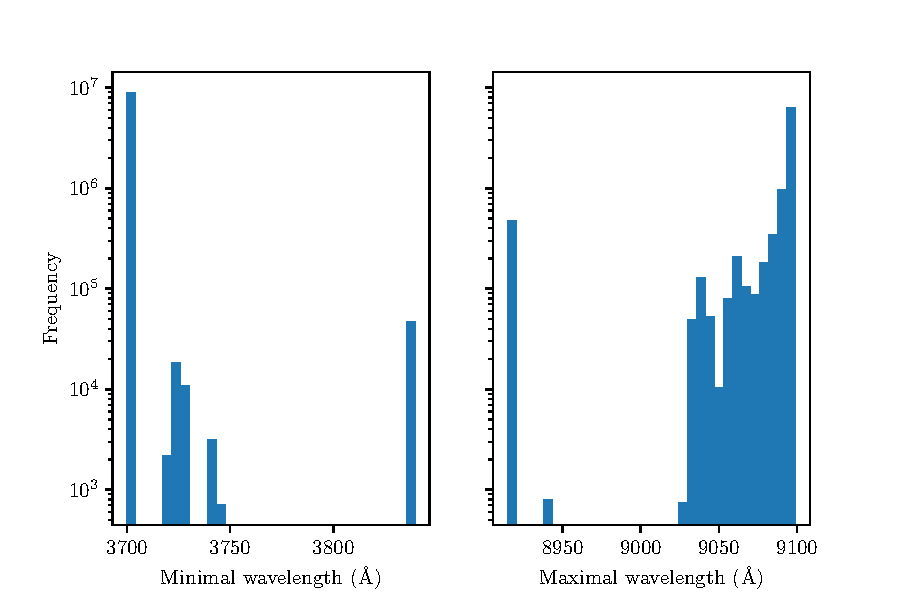
\includegraphics[width=\textwidth]{img/wavemin_wavemax_hist.pdf}
	\caption{Minimal and maximal wavelengths of all LAMOST spectra.}
	\label{wavemin_wavemax_hist}
\end{figure}

Given the selected grid of wavelength we will lose some SDSS spectra
because not all of them have all mesurement in the range.
Figure~\ref{waves_cumulative_hist} shows cumulative histogram of how many spectra we will keep for cuts in different wavelengths.
We see that major drop are behind the selected minimal and maximal wavelengths
that means we will keep most of the spectra.
Precisely, the cut will drop 34\,487 spectra from our source dataset
including 1\,949 spectra of QSO.
Therefore, the source dataset has 4\,816\,713 spectra with 627\,508 spectra of QSOs that can enter a learing of a neural network.

\begin{figure}
	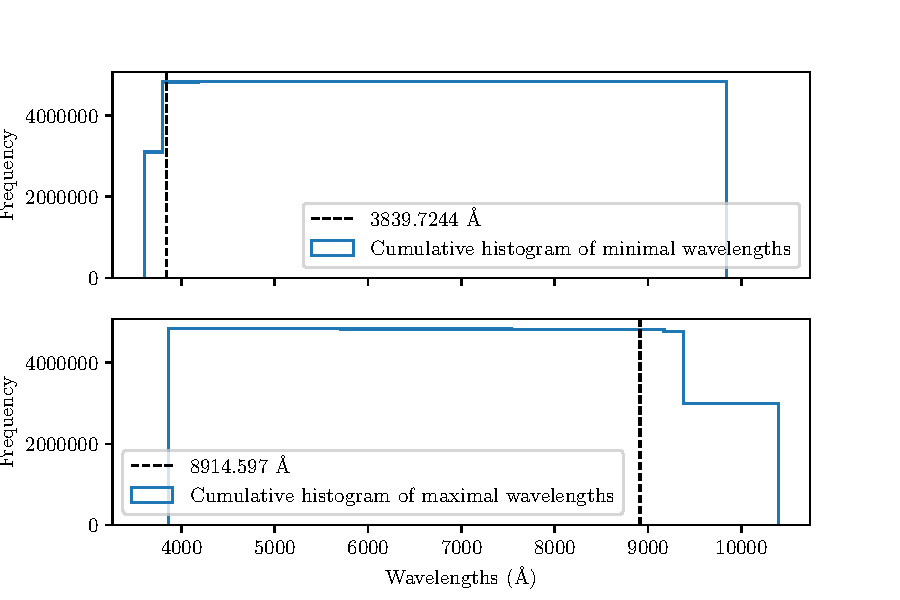
\includegraphics[width=\textwidth]{img/waves_cumulative_hist.pdf}
	% TODO captions of all figures and tables
	\caption{Cutting SDSS specta.}
	\label{waves_cumulative_hist}
\end{figure}

The original sizes of data are unnecessary for experimenting with deep domain adataption on astronomical spectra.
We store each spectrum as a vector of 3\,659 single-precision floating-point number (4 bytes).
The storage setting gives that the SDSS source dataset has about 70.5~GB
and the LAMOST target dataset 132.1~GB.
Data of such size usually cannot fit into memory
and access to a disk significantly slows learning on a GPU.

Therefore, we have subsampled the data to the size of ImageNet~\cite{russakovsky2015}.
We believe that the size of ImageNet is more than reasonable
because ImageNet is the dataset
that enable the superiority of deep neural network in computer vision.
ImageNet has 1 million training examples, 50 thousand validation examples
and 100 thousand testing examples.
Accordingly, we randomly subsampled of source and target datasets
obtaining training sets of size 1 million
and validation sets of size 50 thousand
while the rest of the data serves as testing sets.
We summarise sizes of datasets with corresponding number of QSOs in Table~\ref{datasets_sizes}.
Table~\ref{datasets_sizes} shows a significant class imbalance in the LAMOST DR5
where QSOs are very rare (less then 0.4\%).

\begin{table}
	\begin{center}
	\begin{tabular}{|l|r|r|}
		\hline
		Name & QSOs & Total spectra \\ \hline \hline
		SDSS DR14 & 629\,457 (12.98\%) & 4\,851\,200 \\ \hline
		usable SDSS DR14 & 627\,508 (13.03\%) & 4\,816\,713 \\ \hline
		SDSS training set & 130\,904 (13.09\%) & 1\,000\,000 \\ \hline
		SDSS validation set & 6\,552 (13.10\%) & 50\,000 \\ \hline
		LAMOST DR5 v3 & 31\,755 (0.35\%) & 9\,026\,365 \\ \hline
		LAMOST training set & 3\,517 (0.35\%) & 1\,000\,000 \\ \hline
		LAMOST validation set & 190 (0.38\%) & 50\,000 \\ \hline
	\end{tabular}
	\end{center}
	\caption{Sizes of datasets.}
	\label{datasets_sizes}
\end{table}

The last step of data preparation is min-max scaling of each spectrum into the \([-1; 1]\) range:

\begin{equation}
	\mathbf{x}_i = 2 \frac{\mathbf{x}_i - \min(\mathbf{x}_i)}{
		\max(\mathbf{x}_i) - \min(\mathbf{x}_i)} - 1,
\end{equation}

where \(\mathbf{x}_i \in \mathbb{R}^{3659}\) is a spectrum as defined in Chapter~\ref{da_chapter}
and functions \(\min(\cdot)\) and \(\max(\cdot)\) returns the smallest and the largest element of a given vectore respectively.

There are two benefits of the min-max scaling.
Firstly, the data will be in a suitable range for learning of neural networks
which will stabilise learning.
Secondly, the scaling will remove intensity properties of spectra
leaving us only with the spectrum shape which we are interesting in.

\section{Dimensionality Reduction}

In this section, we investigate the structure of joint data space of source and target datasets with three dimensionality reduction methods:
\textit{principal component analysis},
\textit{t-Distributed Stochastic Neighbor Embedding}
and \textit{Unifrom Maniforld Approximation and Projection} (UMAP).
We would like to get an idea how well are the source and target data mixed together,
if there are some separate clusters or the data are rather continuos.

To avoid visualisation overwhelmed with data points,
we sampled 2\,500 spectra from the source training set
and 2\,500 spectra from the target traininig set.
The spectra are min-max scaled not standardized
because the relation between features are meaningful
and we do not want to supress the relationship.

\textit{Principal component analysis} (PCA) is a simple linear machine learning algorithm
that is used either for visualisation or feature extraction by dimensionality reduction.
PCA learns a representation whose features are uncorrelation with each other
and selects features will the largest variation.~\cite{goodfellow2016}
We show the visualisation obtained with PCA in Figure~\ref{pca}.
The plot shows that source data tent to concenrate in the middle
while the target data are on the edges.
However, there are no regions containing only source or target data.
Moreover, in the middle extending to the right there is a kind of line component.

\begin{figure}
	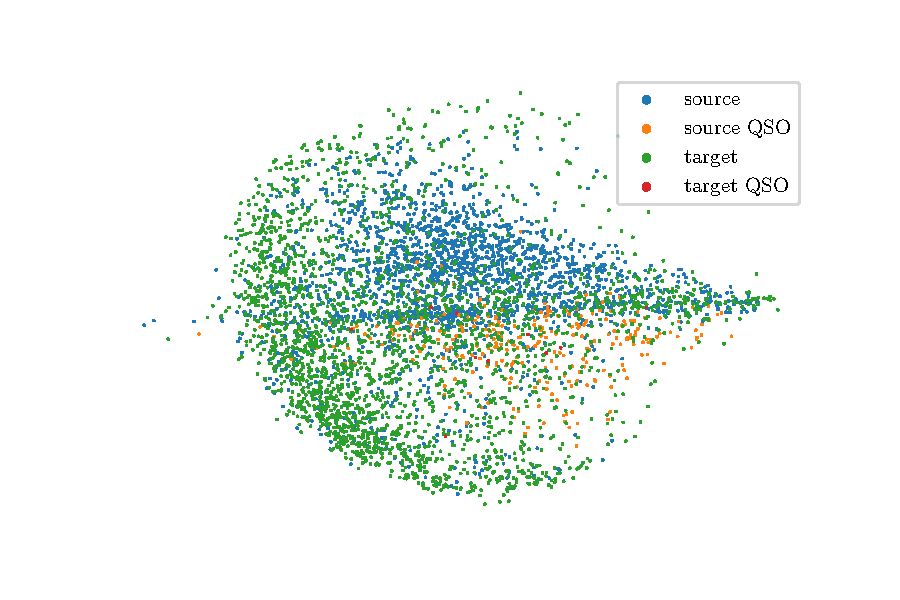
\includegraphics[width=\textwidth]{img/pca.pdf}
	\caption{PCA}
	\label{pca}
\end{figure}

\textit{t-Distributed Stochastic Neighbor Embedding} (t-SNE)~\cite{maaten2008, wattenberg2016} is a popular method for visualisation of high-dimensional data.
The t-SNE method is non-linear, iterative
and peforms different transformation of different regions.
A tunable hyperparemeter of t-SNE is \textit{perplexity}
which is a guess about the number of neighbors of a data point.
Typically, the optimal value is between 5 and 50.

We reduce dimensionality with t-SNE for perplexities from \(\{5, 10, 30, 50, 100\}\).
The best result was for the value 30
and the result is shown in Figure~\ref{tsne}.
The t-SNE embedding have similar structure to the Figure~\ref{pca} of PCA.
There are mostly source data in the center and target data around it.
However the separation between center and edges seems to be bigger.
Still ther is the line component extending to the right.

t-SNE is often used in the papers presenting a deep domain adaptation methods
to show how feature extracted from a higher layer in an adapted network
are better mix when a domain adaptation method is employed.
On the other hand, we a network is not adapted the source and target data
can be easily visually separated in a t-SNE visualisation.

\begin{figure}
	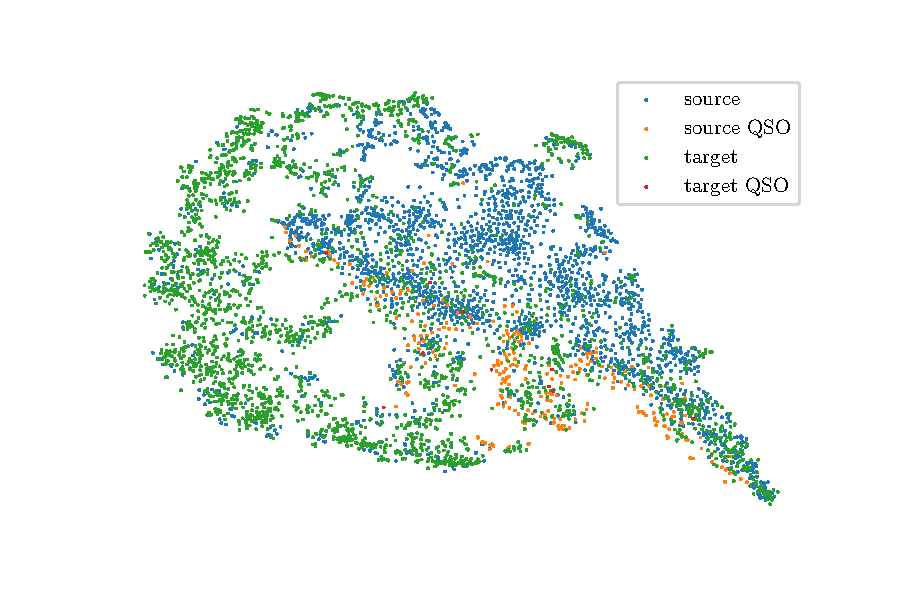
\includegraphics[width=\textwidth]{img/tsne.pdf}
	\caption{t-SNE}
	\label{tsne}
\end{figure}

\textit{Unifrom Manifold Approximation and Projection} (UMAP)~\cite{mcinnes2018}
is a non-linear dimensionality reduction algortihm based on manifold learning and ideas from topological data analysis.
It achieves visualisations similar to t-SNE but it is significantly faster.
Visualisation with UMAP is displayed in Figure~\ref{umap}
and have very similar structure to t-SNE embedding in Figure~\ref{tsne}.

\begin{figure}
	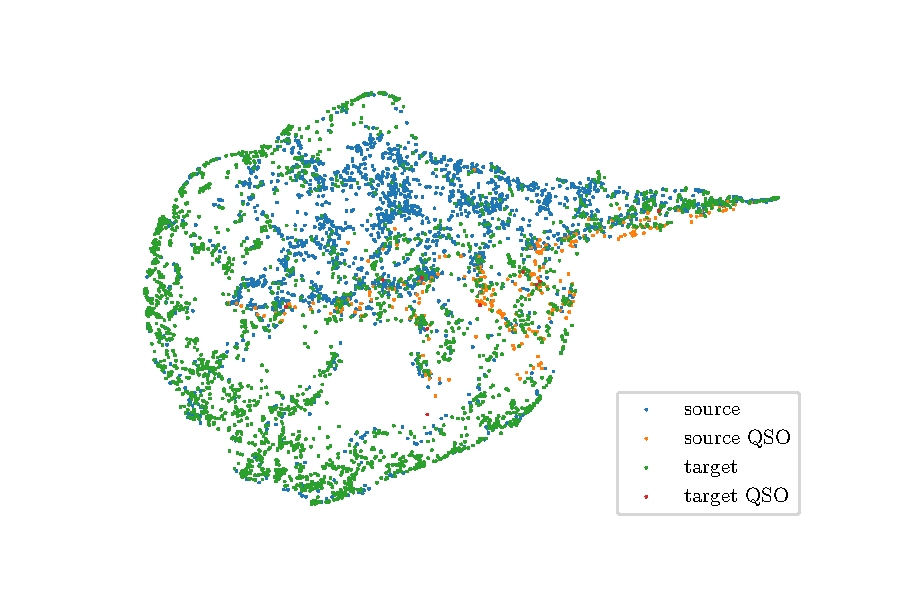
\includegraphics[width=\textwidth]{img/umap.pdf}
	\caption{UMAP}
	\label{umap}
\end{figure}

\section{Baseline: Results without Deep Domain Adapatation}
\label{baseline}

Now, we are ready for training of neural networks
but before we will dive into deep domain adapatation
we will train a classical convulutional network
which will serve as baseline to
which we can compare results of networks augumented with deep domain adaptation.

As the baseline, we choose LeNet-5~\cite{lecun1998} convolutional neural network
which was originaly used to recognize hand written digits
of the MNIST dataset.\footnote{Available from: \url{http://yann.lecun.com/exdb/mnist/}}
We have choosen the architecture of LeNet-5
because it is the simplest model used in the DANN paper~\cite{ganin2016}.
However, the network is design for processing of two-dimensional images
while spectrum is a one-dimensional image.
Therefore, we have to substitude the two-dimensional convolutions with one-dimensional convolutions.
Moreover, we increased the kernel size and stride of pooling layer from 2 to 16
so that the output of the convolutional layer is reasonably big.
If we left the original pooling layer
the input to the first fully connected layer would be of size 43\,872.
in comparison the original input size 768 for the MNIST dataset.
The kernel size and stride of 16 will reduce the input size of our network to 672.
Figure~\ref{lenet} displays the final architecture
which we implemented in PyTorch~\cite{paszke2019}.

\tikzstyle{layer} = [align=center,draw=black,font=\tiny,rectangle,text centered]
\begin{figure}
	\begin{center}
		\subfloat[][LeNet-5]{
			\begin{tikzpicture}[node distance=1.5cm]
				\node (conv1) [layer] {conv1\\5-32\\ReLU};
				\node (pool1) [layer,right of=conv1] {pool1\\16-16};
				\node (conv2) [layer,right of=pool1] {conv2\\5-48\\ReLU};
				\node (pool2) [layer,right of=conv2] {pool2\\16-16};
				\node (fc1) [layer,right of=pool2] {fc1\\100\\ReLU};
				\node (fc2) [layer,right of=fc1] {fc2\\100\\ReLU};
				\node (fc3) [layer,right of=fc2] {fc3\\1\\sigmoid};
				\draw [->] (conv1) -- (pool1);
				\draw [->] (pool1) -- (conv2);
				\draw [->] (conv2) -- (pool2);
				\draw [->] (pool2) -- (fc1);
				\draw [->] (fc1) -- (fc2);
				\draw [->] (fc2) -- (fc3);
			\end{tikzpicture}
			\label{lenet}
		}\\
		\subfloat[][DDC]{
			\begin{tikzpicture}[node distance=1.5cm]
				\node (conv1) [layer] {conv1\\5-32\\ReLU};
				\node (pool1) [layer,right of=conv1] {pool1\\16-16};
				\node (conv2) [layer,right of=pool1] {conv2\\5-48\\ReLU};
				\node (pool2) [layer,right of=conv2] {pool2\\16-16};
				\node (fc1) [layer,right of=pool2] {fc1\\100\\ReLU};
				\node (bottleneck) [layer,right of=fc1,fill=red!50] {bottleneck\\64\\ReLU};
				\node (fc2) [layer,right of=bottleneck] {fc2\\100\\ReLU};
				\node (fc3) [layer,right of=fc2] {fc3\\1\\sigmoid};
				\draw [->] (conv1) -- (pool1);
				\draw [->] (pool1) -- (conv2);
				\draw [->] (conv2) -- (pool2);
				\draw [->] (pool2) -- (fc1);
				\draw [->] (fc1) -- (bottleneck);
				\draw [->] (bottleneck) -- (fc2);
				\draw [->] (fc2) -- (fc3);
			\end{tikzpicture}
			\label{ddc_architecture}
		}\\
		\subfloat[][DANN]{
			\begin{tikzpicture}[node distance=1.5cm]
				\node (conv1) [layer] {conv1\\5-32\\ReLU};
				\node (pool1) [layer,right of=conv1] {pool1\\16-16};
				\node (conv2) [layer,right of=pool1] {conv2\\5-48\\ReLU};
				\node (pool2) [layer,right of=conv2] {pool2\\16-16};
				\node (fc1) [layer,right of=pool2,fill=blue!50] {fc1\\100\\ReLU};
				\node (fc2) [layer,right of=fc1,fill=blue!50] {fc2\\100\\ReLU};
				\node (fc3) [layer,right of=fc2,fill=blue!50] {fc3\\1\\sigmoid};
				\node (grl) [layer,below of=pool2,fill=green!50] {gradient\\reversar\\layer};
				\node (fc4) [layer,right of=grl,fill=green!50] {fc4\\100\\ReLU};
				\node (fc5) [layer,right of=fc4,fill=green!50] {fc5\\1\\sigmoid};
				\draw [->] (conv1) -- (pool1);
				\draw [->] (pool1) -- (conv2);
				\draw [->] (conv2) -- (pool2);
				\draw [->] (pool2) -- (fc1);
				\draw [->] (fc1) -- (fc2);
				\draw [->] (fc2) -- (fc3);
				\draw [->] (pool2) -- (grl);
				\draw [->] (grl) -- (fc4);
				\draw [->] (fc4) -- (fc5);
			\end{tikzpicture}
		}\\
		\subfloat[][DRCN]{
			\begin{tikzpicture}[node distance=1.5cm]
				% encoder
				\node (conv1) [layer] {conv1\\5-32\\ReLU};
				\node (pool1) [layer,right of=conv1] {pool1\\16-16};
				\node (conv2) [layer,right of=pool1] {conv2\\5-48\\ReLU};
				% feature labelling
				\node (pool2) [layer,right of=conv2,fill=blue!50] {pool2\\16-16};
				\node (fc1) [layer,right of=pool2,fill=blue!50] {fc1\\100\\ReLU};
				\node (fc2) [layer,right of=fc1,fill=blue!50] {fc2\\100\\ReLU};
				\node (fc3) [layer,right of=fc2,fill=blue!50] {fc3\\1\\sigmoid};
				% decoder
				\node (conv3) [layer,below of=conv2,fill=green!50] {conv3\\5-48\\ReLU};
				\node (upsample1) [layer,left of=conv3,fill=green!50] {upsample1\\3659};
				\node (conv4) [layer,left of=upsample1,fill=green!50] {conv4\\5-32\\None};
				% connections
				\draw [->] (conv1) -- (pool1);
				\draw [->] (pool1) -- (conv2);
				\draw [->] (conv2) -- (pool2);
				\draw [->] (pool2) -- (fc1);
				\draw [->] (fc1) -- (fc2);
				\draw [->] (fc2) -- (fc3);
				\draw [->] (conv2) -- (conv3);
				\draw [->] (conv3) -- (upsample1);
				\draw [->] (upsample1) -- (conv4);
			\end{tikzpicture}
		}
	\end{center}
	\caption{Architectures}
	\label{lenet_5}
\end{figure}

Furthermore, Donahue et al. showed in the DeCAF (\textit{Deep Convolutional Activation Feature}) paper~\cite{donahue2014}
that features extracted from deep CNN can be repurposed to novel tasks
if the network were trained on a large fixed set in fully supervised fashion.
Meaning that it can be used for domain adaptation on its own.
Therefore, we can expected that our CNN trained on the large SDSS
will be able to find features beneficial for domain adaptation.
Still the DeCAF paper showed that
deep CNN cannnot remove domain bias completelly.
Therefore, there is a space for improvement with deep domain adaptation
and DDC, Deep CORAL and DANN build in experiment on result of DeCAF
because they use AlexNet~\cite{krizhevsky2012} pre-trained on ImageNet dataset.

We trained our adapted LeNet-5 on batches of size 64 for 20 epochs
with the Adam optimiser~\cite{kingma2014} in its default setting
and used the \textit{binary cross entropy loss} defined as:

\begin{equation}
	\mathit{BCE}(\theta) = -\frac{1}{M} \sum_i^M [y_i \log \hat{y}_i + (1 - y_i) \log(1 - \hat{y}_i)],
\end{equation}

where \(\theta\) are all parameters of a model,
\(M\) is the batch size,
\(y_i \in \{0, 1\}\) is the true label
and \(\hat{y}_i \in [0, 1]\) are the model predictions of the \(i\)-th example in the batch.
Furthermore, we intialised the weights and biases in accordance with Xavier initialisation~\cite{glorot2010}.
That is weights of our neural network are sampled from uniform distribution \(\mathcal{U}\):

\begin{equation}
	\mathcal{U}\left(
	-\frac{\sqrt{6}}{\sqrt{\mathit{in} + \mathit{out}}},
	\frac{\sqrt{6}}{\sqrt{\mathit{in} + \mathit{out}}}
	\right),
\end{equation}

where \(\mathit{in}\) is the number of input units of a layer
and \(\mathit{out}\) is the number of output units
and biases are set to zero.

% TODO training progress

\begin{figure}
	\subfloat[][Losses]{
		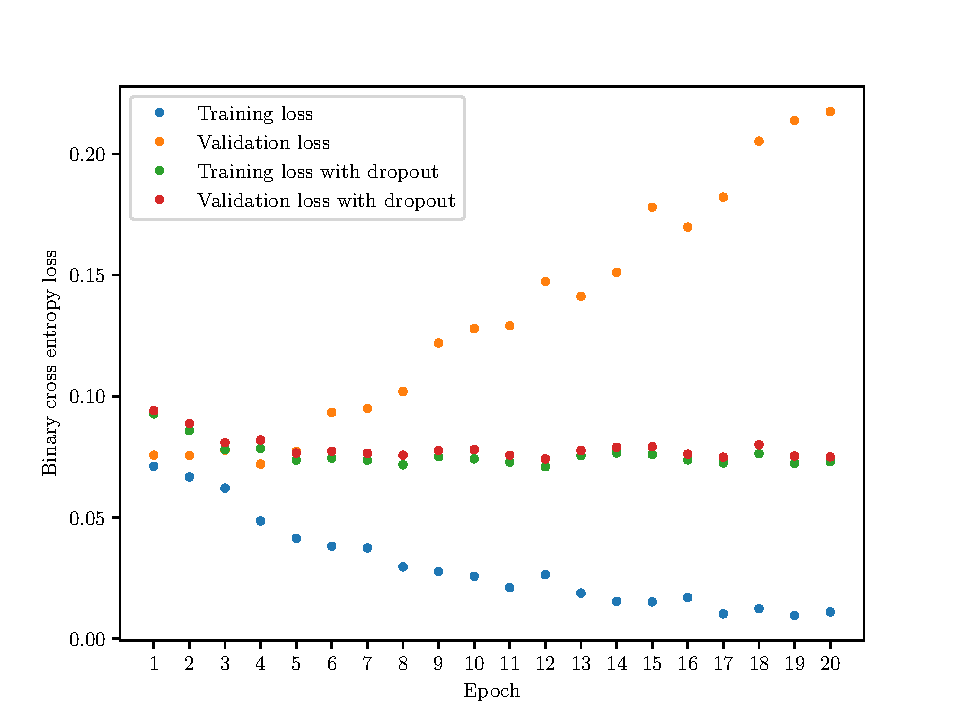
\includegraphics[width=0.5\textwidth]{img/lenet_losses.pdf}
	}
	\subfloat[][\(F_1\) score]{
		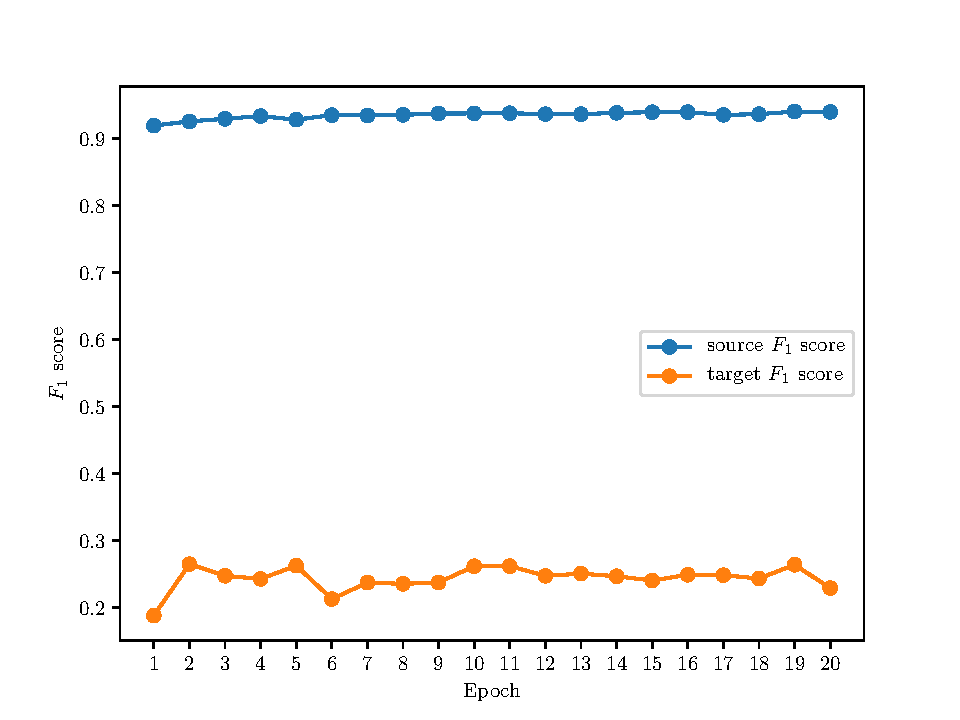
\includegraphics[width=0.5\textwidth]{img/lenet_f1.pdf}
	}
	\caption{Training of LeNet-5}
	\label{lenet_losses}
\end{figure}

% TODO define recall and precision
\textit{Recall} \(r\), \textit{precision} \(p\)
and \textit{\(F_1\) score} is the harmonic mean between \textit{precision} and \textit{recall}:

\begin{align}
	r &= \frac{\mathit{TP}}{\mathit{TP} + \mathit{FN}}, \\
	p &= \frac{\mathit{TP}}{\mathit{TP} + \mathit{FP}}, \\
	F_1 &= \frac{2}{r^{-1} + p^{-1}} = 2 \frac{r p}{r + p},
\end{align}

where \(r\) is recall and \(p\) is precision.
When precision and recall are perfect
\(F_1\) score reaches its best value one and at worst can be zero.

% TODO result evaluation
\(F_1\) score of source is 0.9397 and target 0.2294.
Target precision is is 13.48\% and target recall 76.84\%.

\begin{table}
	\begin{center}
	\subfloat[][Source confusion matrix]{
		\begin{tabular}{|l|r|r|}
			\hline
			Predicted class & \multicolumn{2}{c|}{Actual class} \\ \hline \hline
			& QSO & non-QSO \\ \hline
			QSO & 6\,278 & 532  \\ \hline
			non-QSO & 274 & 42\,916 \\ \hline
		\end{tabular}
	}
	\subfloat[][Target confusion matrix]{
		\begin{tabular}{|l|r|r|}
			\hline
			Predicted class & \multicolumn{2}{c|}{Actual class} \\ \hline \hline
			& QSO & non-QSO \\ \hline
			QSO & 146 & 937 \\ \hline
			non-QSO & 44 & 48\,873 \\ \hline
		\end{tabular}
	}
	\end{center}
\end{table}

% TODO feature t-SNE

\section{Experiments with Deep DA}

Apply domain adaptation to the selected data.

\subsection{DDC: Deep Domain Confusion}

Theory behind DDC is explained in Subsection~\ref{discrepancy_da}.
We followed the same procedure to choose the placement and width
of the adaptation layer as in the DDC paper~\cite{tzeng2014}.

Firstly, we took the LeNet-5 trained in previous Section~\ref{baseline}
and extracted features from the first and second fully-connected layer
(the last fully-connected layer has a trivial width)
for all validation examples.
Then, we computed MMD between the source and target data at each layer with the extracted features.
The MMD at the first fully-connected layer is 50.70
while at the second fully-connected layer is 53.33.
Therefore, we will place the adaptation layer after the first fully-connected layer.

Secondly, we have to optimise the width of the adapataion layer.
Therefore, we trained the LeNet with the adapation layer of sizes
from \(\{4, 8, 16, 32, 64\}\) excluding the low width 2,
not exceeding the output size of previous layer
and stepping by power of two as in the original paper.
Figure~\ref{adaptation_layer} plots the resulting MMD values for different setting and shows that the width 64 is the best.

\begin{figure}
	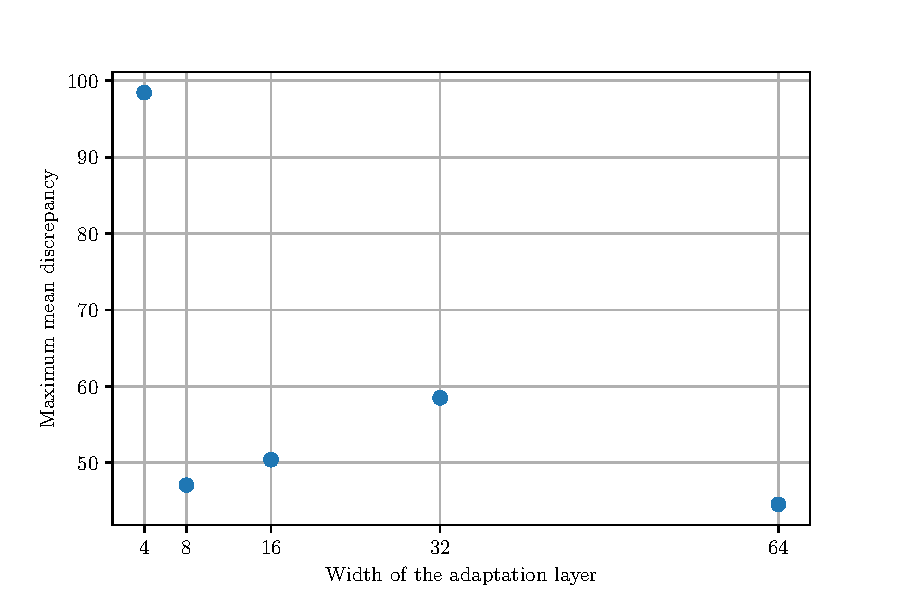
\includegraphics[width=\textwidth]{img/adaptation_layer_width.pdf}
	\caption{Width of the adapation layer}
	\label{adaptation_layer}
\end{figure}

The final architecture of our DDC network is in Figure~\ref{ddc_architecture}. We set the trade-off parameter between the binary cross entropy loss and the MMD loss \(lambda\) to 0.25 as in the DDC experiments
and trained the network in the same way
as described in previous section~\ref{baseline}.

\subsection{Deep CORAL: Deep Correlation Alignment}

\subsection{DANN: Domain-Adversarial Neural Networks}

\subsection{DRCN: Deep Reconstruction-Classification Networks}

\section{Evaluation of Experiments}

Prepare visualisation of results.
